\documentclass[a5paper, 12pt]{scrartcl}

\usepackage{mystyle}
\usepackage[europeanresistors]{circuitikz}
\usepackage{siunitx}

\usepackage{scrlayer-scrpage}

\clearpairofpagestyles{}

\setkomafont{pageheadfoot}{\sffamily\footnotesize}
\setkomafont{pagination}{}

\ohead{Seite~\pagemark}
\ihead{Emil Slomka, Tim Hilt}

\KOMAoptions{
  % chapterprefix=true,
  headsepline=true,
}

\title{Formelsammlung Elektronik}
\author{Emil Slomka, Tim Hilt}

\begin{document}
\newgeometry{left=1cm, right=1cm, top=2cm}
\maketitle

\section{Grundlagen und Wiederholung}

\subsection{Übertragungsfunktion}
\begin{align*}
  F = \frac{U_a}{U_e} = \frac{\text{Widerstände parallel zum Ausgang}}{\text{Widerstände parallel zum Eingang}}
\end{align*}

\mybfcol{Bei Berechnung zweier, paralleler Widerstände \(R_1\) und \(R_2\):}

\begin{align*}
  R_1 || R_2 = \frac{R_1 \cdot R_2}{R_1 + R_2}
\end{align*}

Leistung: \dotfill \(P = \quad \frac{U^2}{R} \quad = \quad U \cdot \frac{U}{R} \quad = \quad U \cdot I\)\\
Zeitkonstante \(\tau\) beim \mybfcol{Kondensator}: \dotfill \(\tau = R \cdot C\)\\
Zeitkonstante \(\tau\) bei der \mybfcol{Spule}: \dotfill \(\tau = \frac{L}{R}\)\\

\begin{figure}[H]
  \centering
  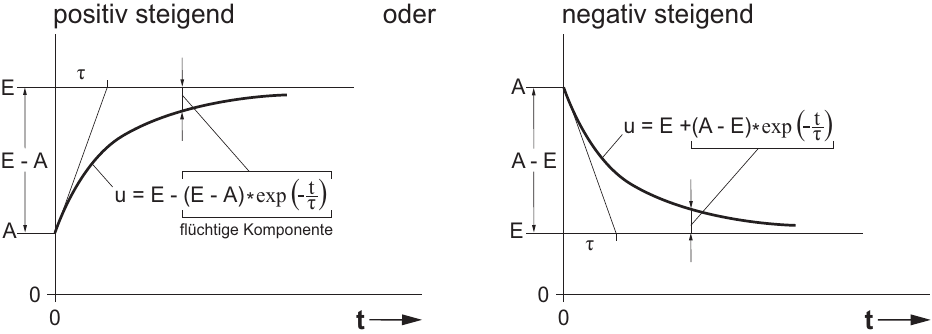
\includegraphics[width=.7\textwidth]{LadekurveKondensator}
  \caption{Ladekurven Kondensator \mybfcol{Achtung: \(t = \Delta t = t_1 - t_0\)}}
\end{figure}

\mybfcol{Achtung: Immer alle Widerstände parallel und in Reihe zum Kondensator berücksichtigen und Übertragungsfunktion für Ladeziel verwenden!}

\begin{center}
  \begin{tabular}{c|c|c|c}
    \toprule
    \(t=\tau\) & \(\approx 63\%\) von\ \(|A-E|\) & \(\rightarrow |A-E| \cdot 0.63\) beim Aufladen & \(\rightarrow |A-E| \cdot 0.37\) beim Entladen\\
    \(t=2\tau\) & \(\approx 86\%\) von\ \(|A-E|\) & \(\rightarrow |A-E| \cdot 0.86\) beim Aufladen & \(\rightarrow |A-E| \cdot 0.14\) beim Entladen\\
    \(t=5\tau\) & \(\approx 99\%\) von\ \(|A-E|\) & \(\rightarrow \approx E\) beim Aufladen & \(\rightarrow \approx A\) beim Entladen\\
    \bottomrule
  \end{tabular}
\end{center}

\begin{figure}[H]
  \centering
  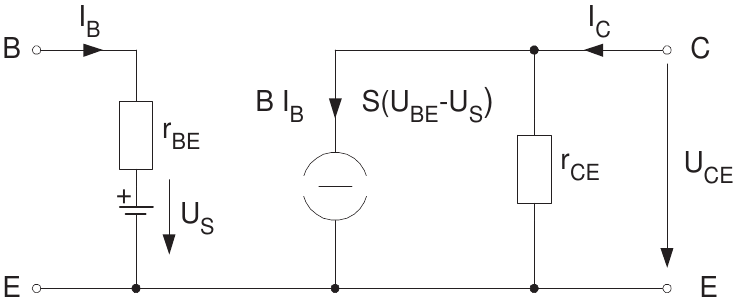
\includegraphics[width=.6\textwidth]{ESBTransistor}
  \caption{Gleichstromersatzschaltbild eines Bipolartransistors}
\end{figure}

\section{Filter}

Im Fourierbereich: \(\omega = 2 \pi f\), im Laplacebereich: \(j\omega = p\)

\begin{table}[H]
  \centering
  \begin{tabular}{cllll}
    & \textbf{RC-Tiefpass} & \textbf{RC-Hochpass} & \textbf{RL-Tiefpass} & \textbf{RL-Hochpass}\\
    \midrule
    \textbf{Übertragungsfunktion \(\frac{U_a}{U_e} = H(j\omega)\)} & \(\frac{1}{1 + j\omega R C}\) & \(\frac{j\omega RC}{1 + j\omega RC}\) & \(\frac{R}{R + j \omega L}\)& \(\frac{j\omega L}{R + j \omega L}\) \\[1em]
    \textbf{Grenzfrequenz \(f_G / \omega_G\)} & \(\frac{1}{2 \pi R C}; \frac{1}{RC}\) & \(\frac{1}{2 \pi R C}; \frac{1}{RC}\) & \(\frac{R}{2 \pi L}; \frac{R}{L}\) & \(\frac{R}{2 \pi L}; \frac{R}{L}\)
  \end{tabular}
  \caption{Grenzfrequenz und Übertragungsfunktionen}
\end{table}

Dämpfung bei passiven Filtern erster Ordnung:

\begin{itemize}
\item \SI{0}{\decibel} im Durchlassbereich
\item \SI{3}{\decibel} an der Grenzfrequenz \(f_G\)
\item \SI{6}{\decibel} pro Oktave (doppelte Frequenz) im Sperrbereich
\item \SI{20}{\decibel} pro Dekade (zehnfache Frequenz) im Sperrbereich
\end{itemize}

\end{document}


%%% Local Variables:
%%% mode: latex
%%% TeX-master: t
%%% End:
